\documentclass[10pt]{beamer}

% ------------------------------------------------------------------------
% Carga del preámbulo personalizado
% (Asegúrate de contar con preamble.tex en la misma carpeta,
%  donde defines temas, colores, macros como \myfront, etc.)
% ------------------------------------------------------------------------
\usetheme[progressbar=frametitle]{metropolis}
\usepackage{appendixnumberbeamer}
\usepackage{fancyvrb}
\usepackage{booktabs}
\usepackage[scale=2]{ccicons}
\usepackage{pgfplots}
\usepgfplotslibrary{dateplot}
\usepackage{type1cm}
\usepackage{lettrine}
\usepackage{ragged2e}
\usepackage{xspace}
\newcommand{\themename}{\textbf{\textsc{metropolis}}\xspace}
\usepackage{graphicx} % Allows including images
\usepackage{booktabs} % Allows the use of \toprule, \midrule and \bottomrule in tables
\usepackage[utf8]{inputenc} %solucion del problema de los acentos.
\usepackage{xcolor}
\definecolor{LightGray}{gray}{0.9}

\usepackage{minted}
\usemintedstyle{tango}
\newcommand{\mypyfile}[1]{\inputminted[linenos=true, fontsize=\footnotesize, frame=lines, framesep=5\fboxrule,framerule=1pt]{python}{#1}}

\setminted[python]{breaklines,frame=lines,framesep=2mm,baselinestretch=1.2,bgcolor=LightGray,linenos, fontsize=\footnotesize} % obeytabs=true, tabsize=2, showtabs=true}

%%%%%%%%%%%%%%%%%%%%%%%%%%%%%%%%%%%%%%%%%%%%%%%%%%%%%%%%%%%%%%%%%%%%%%%%%%%%%%%%%%%%%%
\setbeamercolor{progress bar}{fg=blue!50!black,bg=white!50!black}
\setbeamercolor{title separator}{fg=red!50!black,bg=white!50!black}
\setbeamercolor{frametitle}{fg=white!80!black,bg=red!50!black}
\title[PCFI161]{Programaci\'on para F\'isica y Astronom\'ia}
\subtitle{Departamento de Física.}

\newcommand{\myfront}{
\author[PCFI161]{Corodinadora: C Loyola \\ Profesoras/es C Loyola / C Femenías / Y Navarrete / C Ruiz}
\institute[UNAB]{Universidad Andrés Bello}
\date{Primer Semestre 2025}
}

\titlegraphic{%
  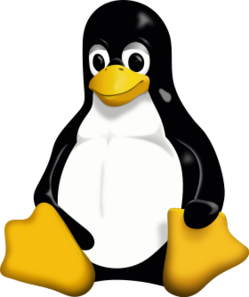
\includegraphics[width=.08\textwidth]{logo-tux.png}\hfill
  
\includegraphics[width=.3\textwidth]{logo-unab.png}\hfill
  
\includegraphics[width=.08\textwidth]{logo-python.png}
}

\makeatletter
\setbeamertemplate{title page}{
  \begin{minipage}[b][\paperheight]{\textwidth}
    \vfill%
    \ifx\inserttitle\@empty\else\usebeamertemplate*{title}\fi
    \ifx\insertsubtitle\@empty\else\usebeamertemplate*{subtitle}\fi
    \usebeamertemplate*{title separator}
    \ifx\beamer@shortauthor\@empty\else\usebeamertemplate*{author}\fi
    \ifx\insertdate\@empty\else\usebeamertemplate*{date}\fi
    \ifx\insertinstitute\@empty\else\usebeamertemplate*{institute}\fi
    \vfill
    \ifx\inserttitlegraphic\@empty\else\inserttitlegraphic\fi
    \vspace*{1cm}
  \end{minipage}
}
\makeatother


\makeatletter
\setlength{\metropolis@titleseparator@linewidth}{2pt}
\setlength{\metropolis@progressonsectionpage@linewidth}{2pt}
\setlength{\metropolis@progressinheadfoot@linewidth}{2pt}
\makeatother


\begin{document}

% ------------------------------------------------------------------------
% Portada personalizada, en tu preamble.tex podrías definirla con \myfront
% ------------------------------------------------------------------------
\myfront{}


% ------------------------------------------------------------------------
% Slide 1: Portada
% ------------------------------------------------------------------------
\begin{frame}
  \titlepage
\end{frame}

% ------------------------------------------------------------------------
% Slide 2: Índice / Tabla de contenidos
% ------------------------------------------------------------------------
\begin{frame}
  \frametitle{Resumen - Sesión 1 (Semana 1)}
  \tableofcontents
\end{frame}

% ----------------------------------------------------------------------------------------
% Configuración de bloques en Metropolis (u otra) si corresponde
% ----------------------------------------------------------------------------------------
\metroset{block=fill}

% ----------------------------------------------------------------------------------------
% SECCIÓN 1: Contexto e Introducción
% ----------------------------------------------------------------------------------------
\section{Contexto del curso e Introducción}

%\textcolor{DarkPythonBlue}{Contexto e Introducción}

% ------------------------------------------------------------------------
% Slide 3: Contexto del Curso
% ------------------------------------------------------------------------
\begin{frame}{Contexto del Curso}
  \begin{itemize}
    \item \textbf{Asignatura:} Programación para la Física y Astronomía.
    \item \textbf{Período:} 1er semestre (de acuerdo al Syllabus).
    \item \textbf{Objetivo principal de esta sesión:}
      \begin{itemize}
        \item Presentación de Syllabus Oficial
        \item Introducir las herramientas fundamentales del curso.
        \item Familiarizarnos con el entorno de programación (Python, Google Colab).
      \end{itemize}
    \item Corresponde a la \textbf{Sesión 1, Semana 1}.
  \end{itemize}
\end{frame}

% ------------------------------------------------------------------------
% Slide 4: ¿Por qué Programación en Física y Astronomía?
% ------------------------------------------------------------------------
\begin{frame}{¿Por qué Programar en Física y Astronomía?}
  \begin{itemize}
    \item Muchas áreas de la Física y Astronomía requieren simulaciones y análisis de grandes volúmenes de datos.
    \item Python se ha vuelto esencial para:
      \begin{itemize}
        \item Resolver problemas numéricos complejos.
        \item Procesar y visualizar datos (observacionales o experimentales).
        \item Facilitar la reproducibilidad de la investigación.
      \end{itemize}
    \item Además, tiene una enorme comunidad científica activa.
  \end{itemize}
\end{frame}

% ------------------------------------------------------------------------
% Slide 5: Breve Vista al Syllabus
% ------------------------------------------------------------------------
\begin{frame}{Breve Vista al Syllabus}
  \begin{itemize}
    \item \textbf{Unidad I:} Elementos Básicos (GNU/Linux, Google Colab, Python).
    \item \textbf{Unidad II:} Programación en Python (tipos, aritmética, funciones).
    \item \textbf{Unidad III:} Controladores y arreglos (if, while, for, listas, slicing).
    \item \textbf{Unidad IV:} Gráficas con Matplotlib.
    \item \textbf{Unidad V:} Manejo de datos (clases, estadística, NumPy/Pandas).
    \item \textbf{Unidad VI:} Algoritmos y Performance (sorting, recursividad, hilos, etc.).
  \end{itemize}

\begin{block}{Syllabus 2025}
Vamos entonces a revisar el detalle del Syllabus de este período.
\end{block}
\end{frame}

% ----------------------------------------------------------------------------------------
% SECCIÓN 2: Herramientas Principales
% ----------------------------------------------------------------------------------------
\section{Herramientas Principales}

% ------------------------------------------------------------------------
% Slide 6: Google Colab
% ------------------------------------------------------------------------
\begin{frame}{Google Colab}
  \begin{itemize}
    \item Plataforma online gratuita de Google para programar en Python.
    \item \textbf{Ventajas:}
      \begin{itemize}
        \item No requiere instalación local.
        \item Integrada con Google Drive (colaboración sencilla).
        \item Ejecución en la nube (libera recursos locales).
      \end{itemize}
    \item Sólo necesitas una cuenta de Google.
  \end{itemize}
  \vspace{0.3cm}
  \textbf{Nota:} Otras alternativas incluyen Jupyter, VSCode, etc.

  \begin{block}{IMPORTANTE!!!}
    El que nuestro curso sea de programación, es \textbf{altamente recomendado} que cada estudiante tenga su propio cuaderno, en donde vamos a anotar cosas importante a medida que las clases avancen.
  \end{block}
\end{frame}

\begin{frame}{Creación de un Notebook en Colab}
  \begin{enumerate}
    \item Visita: \texttt{https://colab.research.google.com}
    \item Inicia sesión con tu cuenta de Google.
    \item Crea un nuevo cuaderno (\emph{New Notebook}).
    \item Almacena el archivo en tu Google Drive.
  \end{enumerate}
  \textbf{Sugerencia:} Organiza tus carpetas en Drive para mantener un buen orden.
\end{frame}


% ------------------------------------------------------------------------
% Slide 6.1: Tutorial Google Colab - Paso a Paso
% ------------------------------------------------------------------------
\begin{frame}
  \frametitle{Google Colab - Tutorial Paso a Paso}
  \begin{center}
    \textbf{Paso 1: Acceso inicial a Google Colab}
  \end{center}
  \begin{figure}
    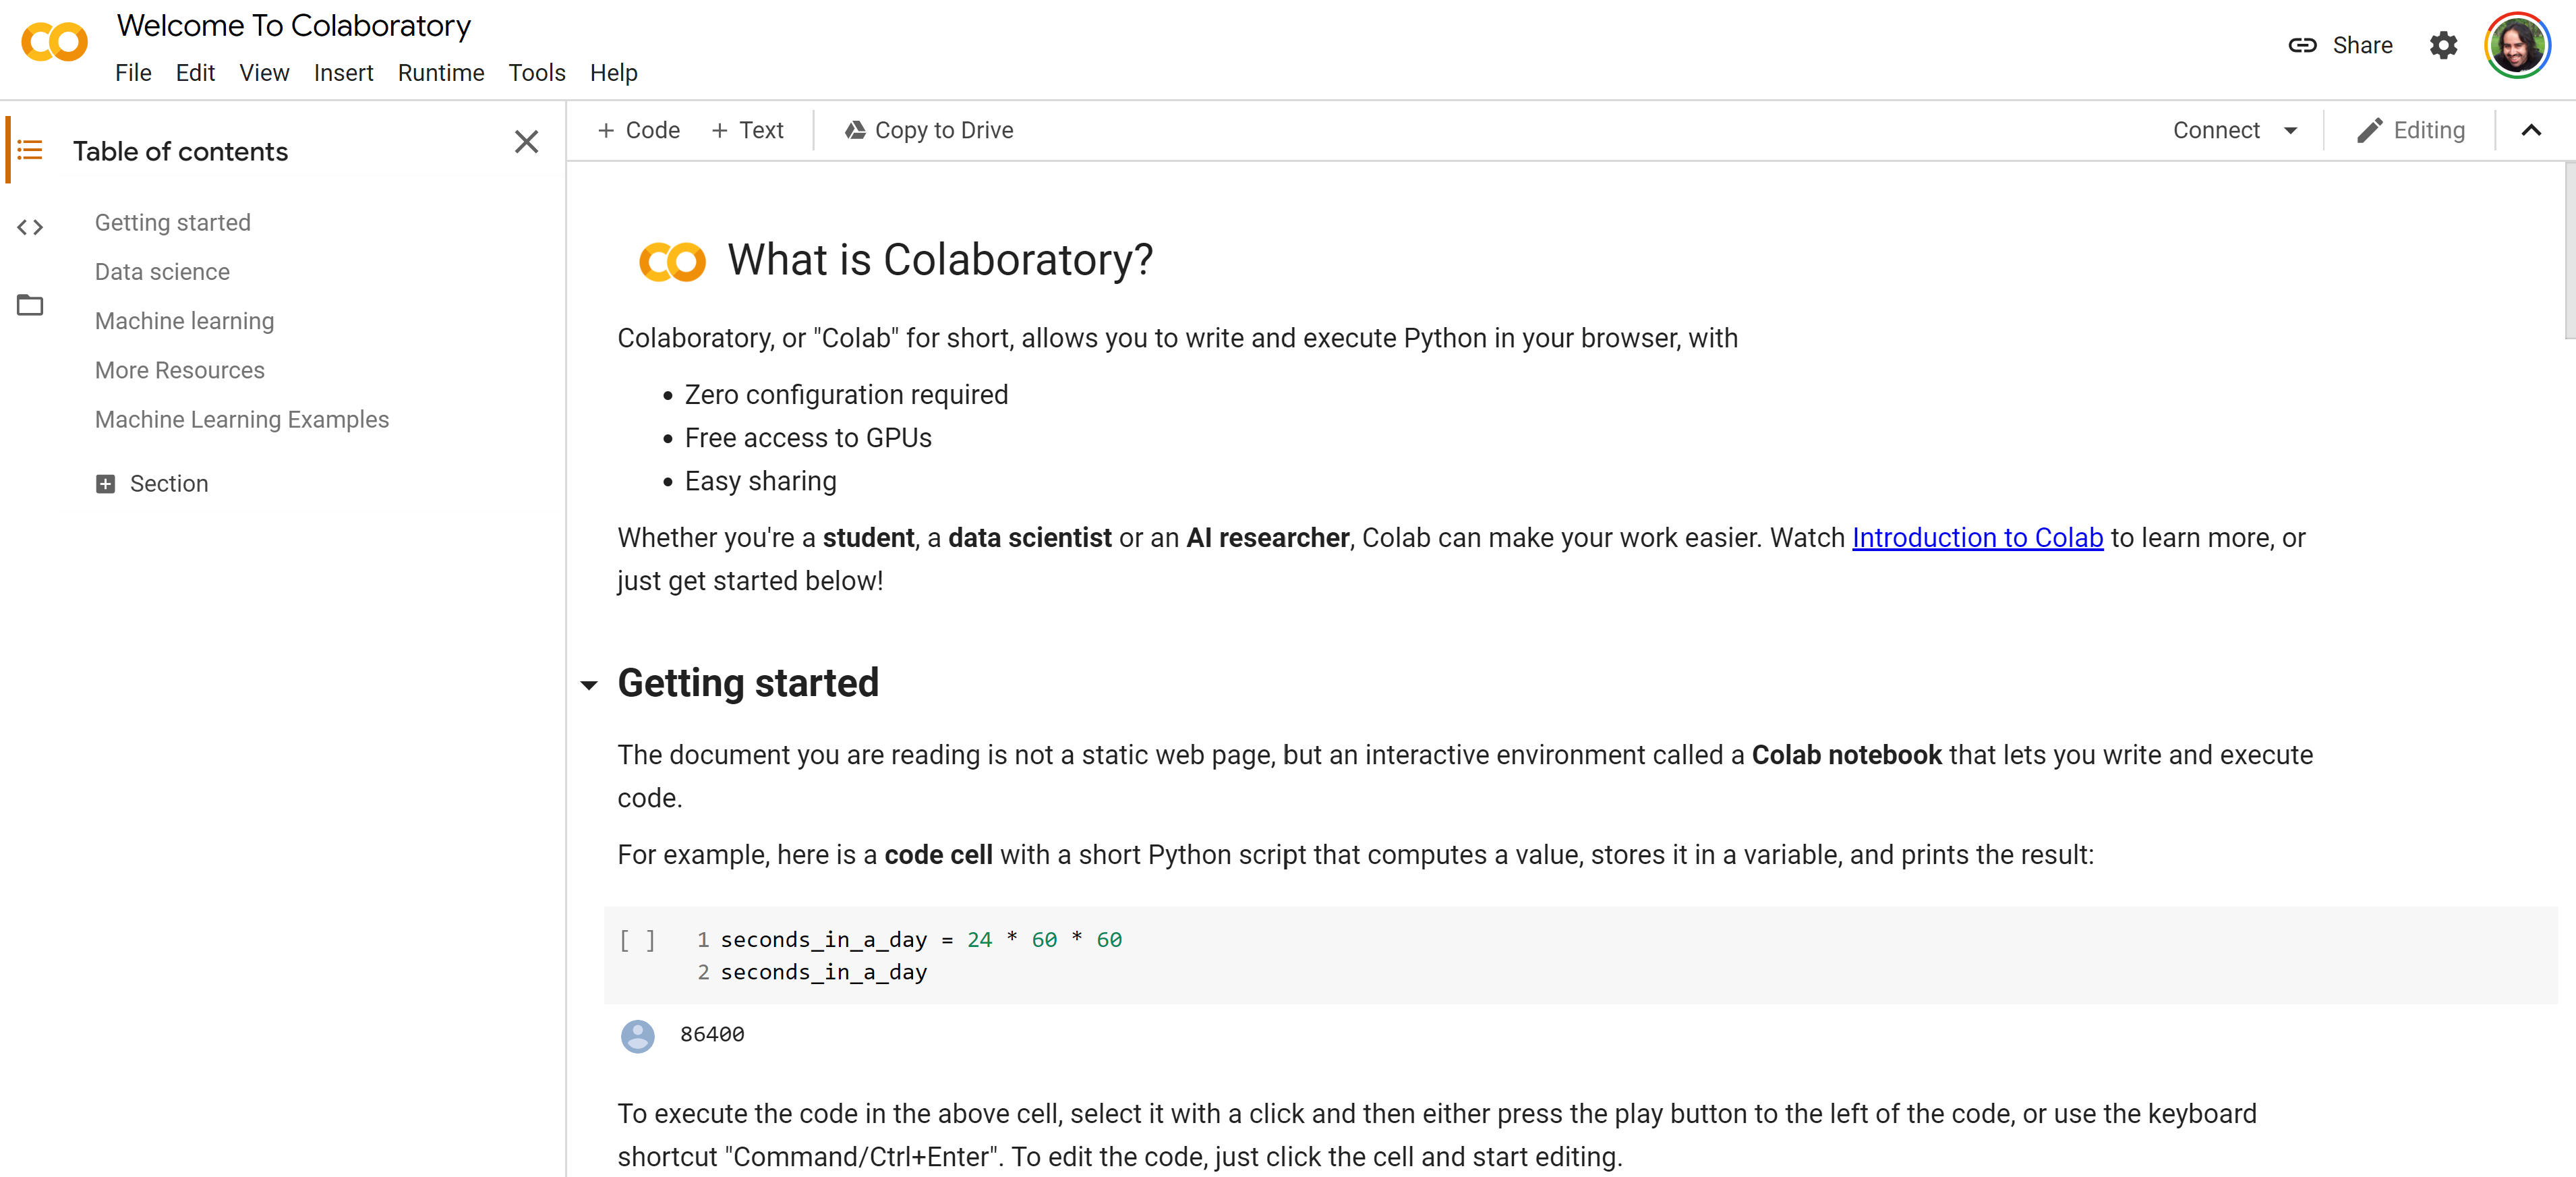
\includegraphics[width=0.95\textwidth]{2) Colab/GColab01.png}
  \end{figure}
\end{frame}

\begin{frame}
  \frametitle{Google Colab - Tutorial Paso a Paso}
  \begin{center}
    \textbf{Paso 2: Creación de nuevo notebook}
  \end{center}
  \begin{figure}
    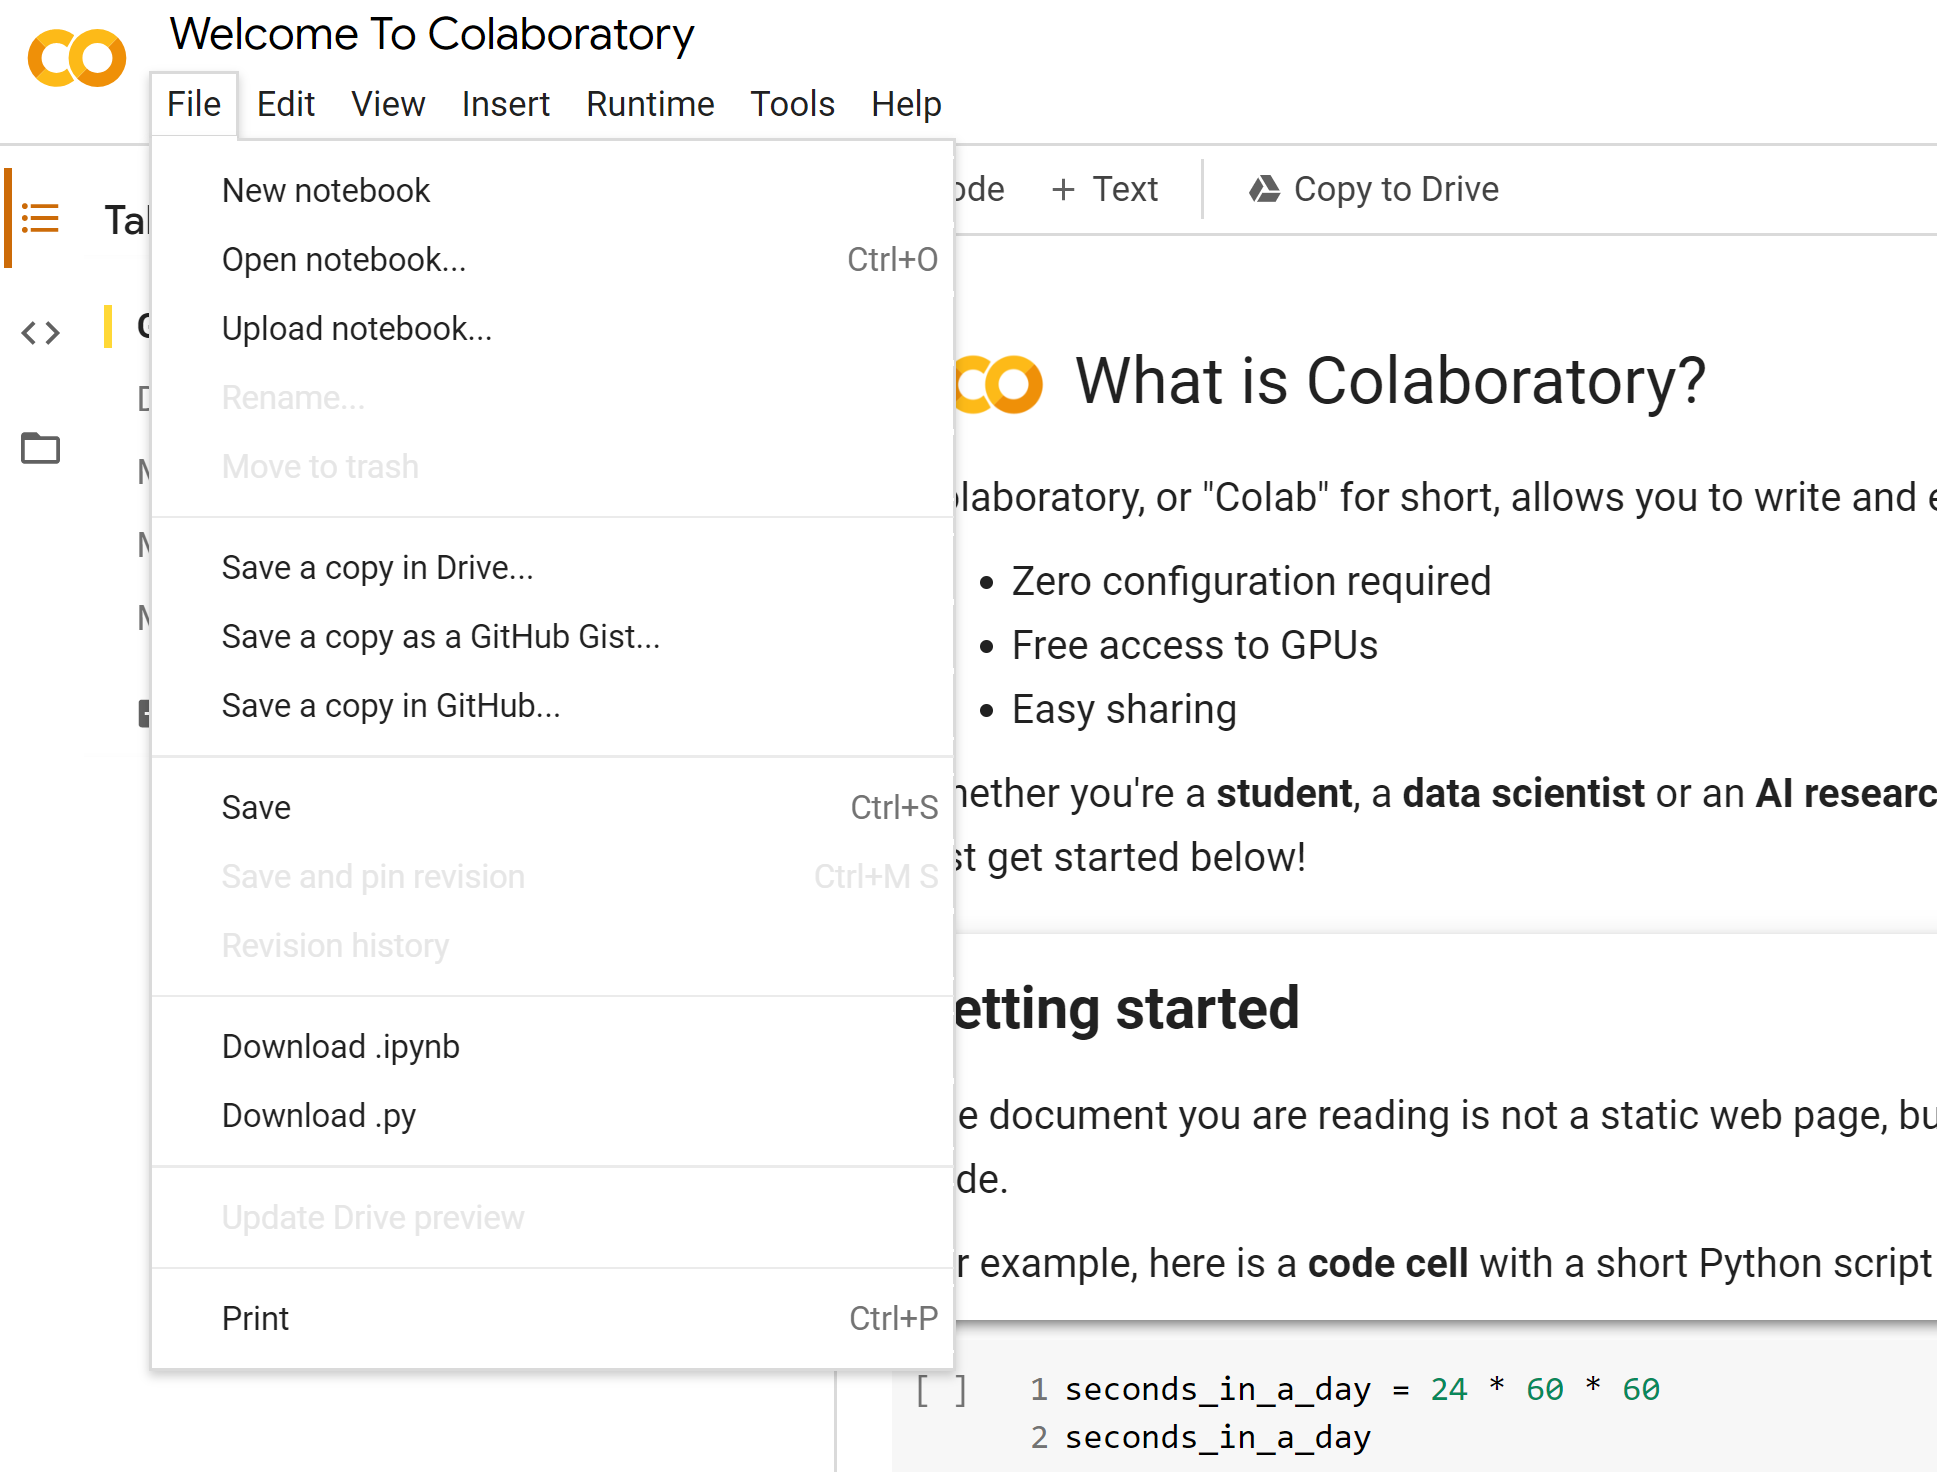
\includegraphics[width=0.95\textwidth]{2) Colab/GColab02.png}
  \end{figure}
\end{frame}

\begin{frame}
  \frametitle{Google Colab - Tutorial Paso a Paso}
  \begin{center}
    \textbf{Paso 3: Donde guardar el notebook}
  \end{center}
  \begin{figure}
    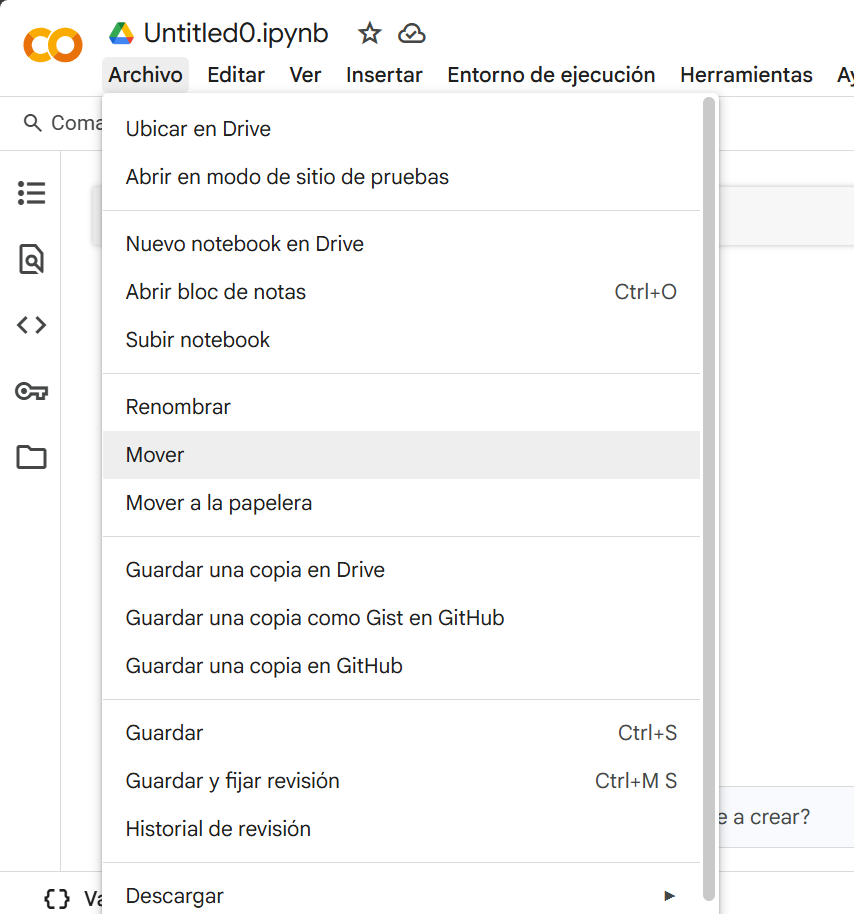
\includegraphics[width=0.95\textwidth]{2) Colab/GColab03.png}
  \end{figure}
\end{frame}

\begin{frame}
  \frametitle{Google Colab - Tutorial Paso a Paso}
  \begin{center}
    \textbf{Paso 4: Empezar a crear carpetas}
  \end{center}
  \begin{figure}
    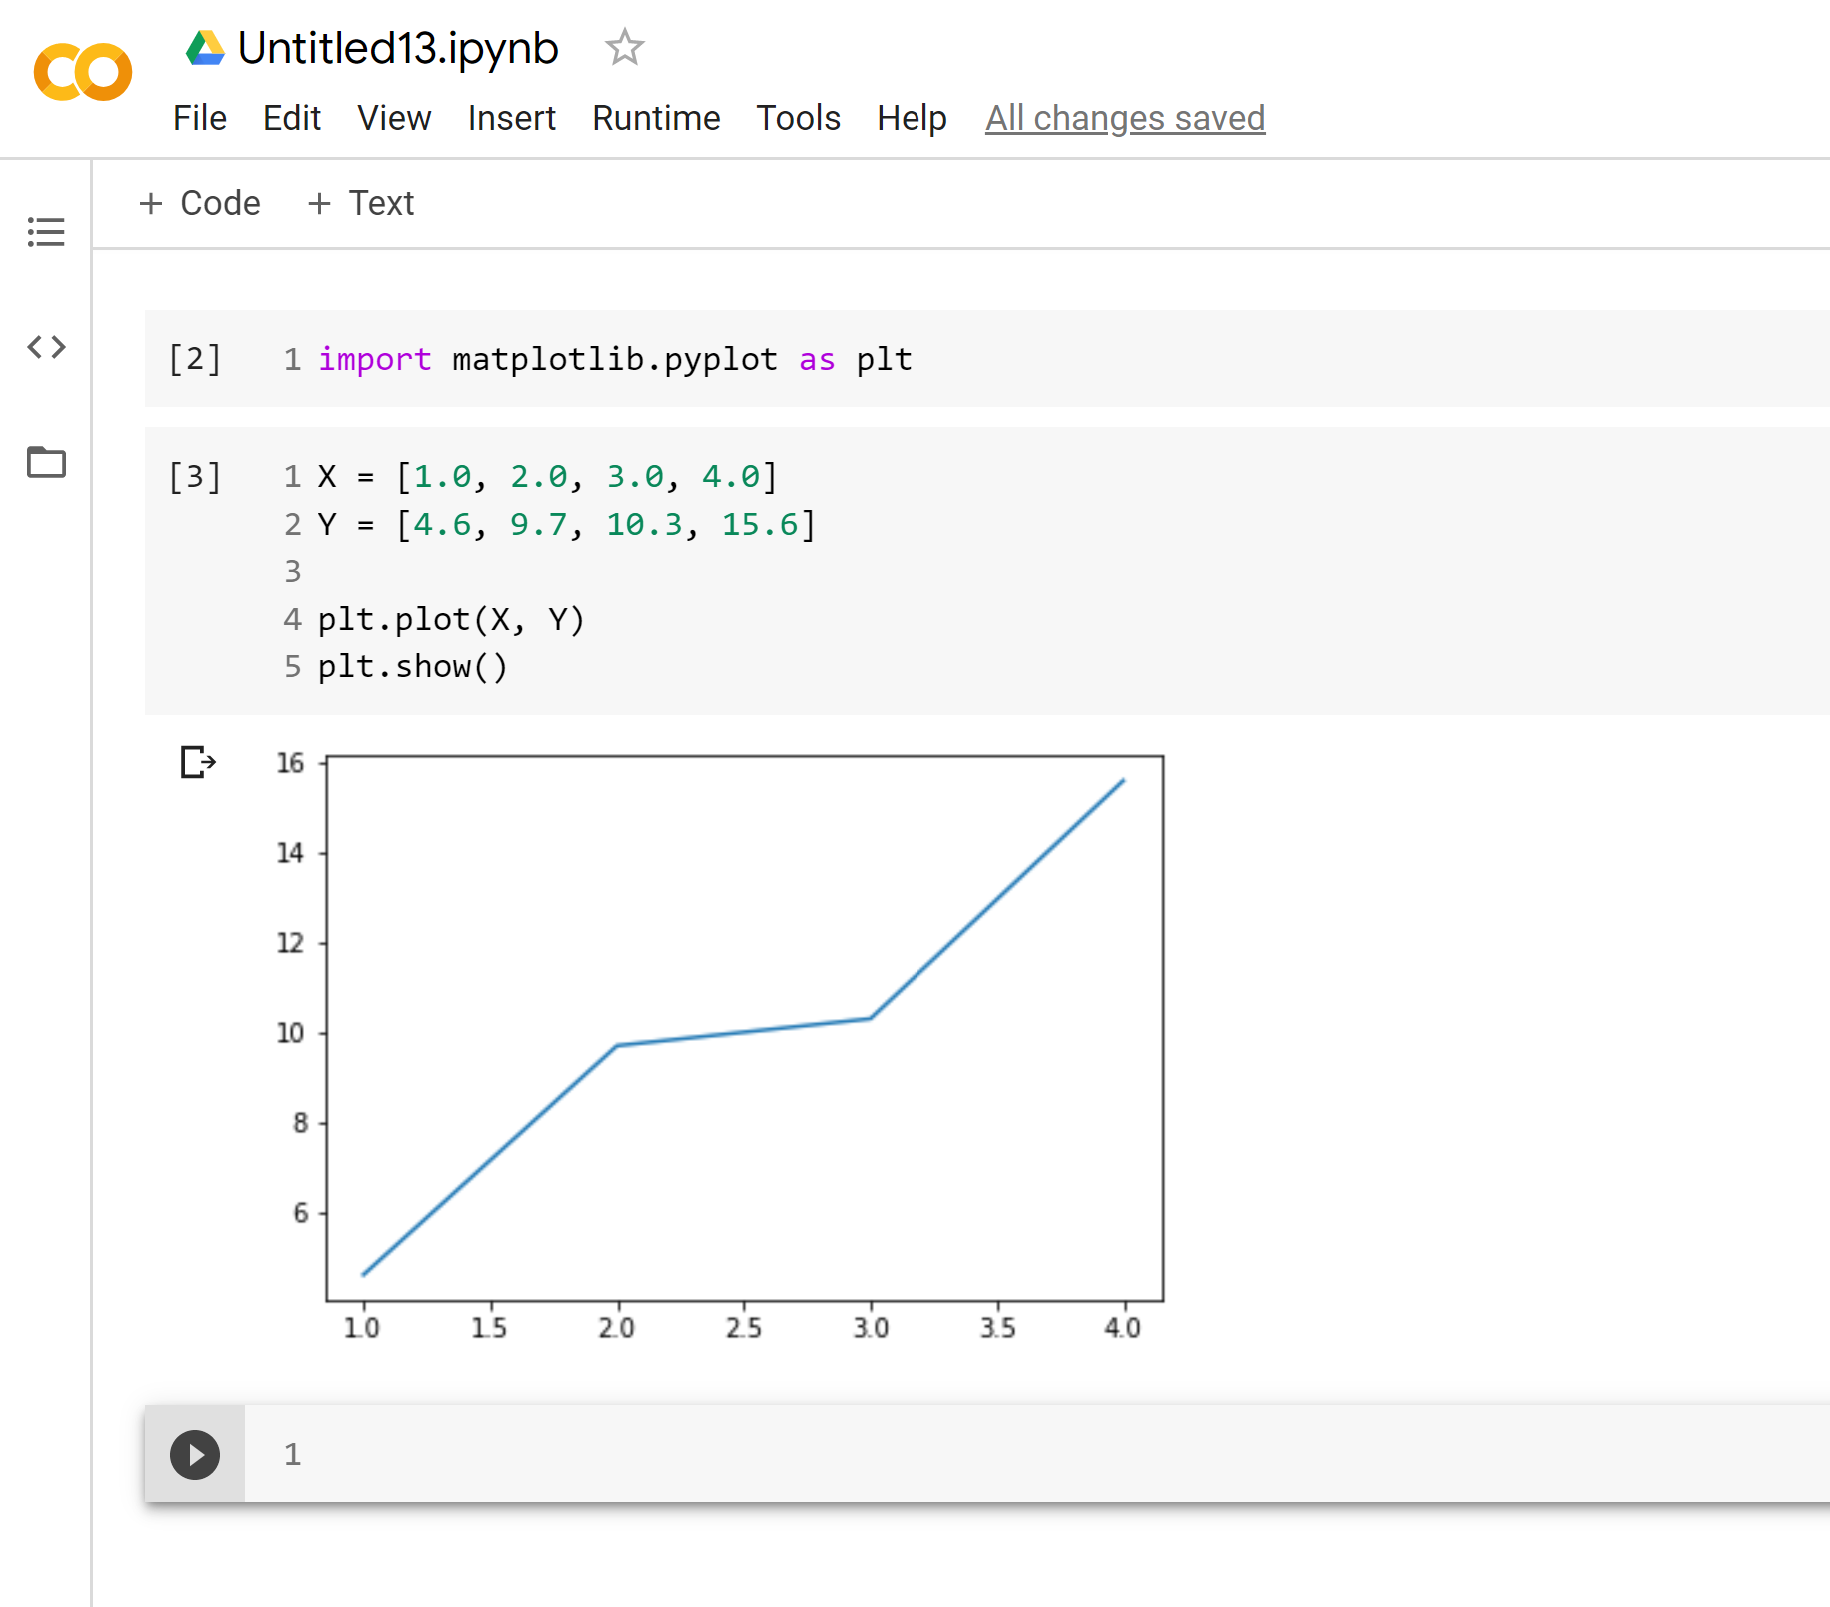
\includegraphics[width=0.95\textwidth]{2) Colab/GColab04.png}
  \end{figure}
\end{frame}

\begin{frame}
  \frametitle{Google Colab - Tutorial Paso a Paso}
  \begin{center}
    \textbf{Paso 5: Crear carpeta con nombre del curso}
  \end{center}
  \begin{figure}
    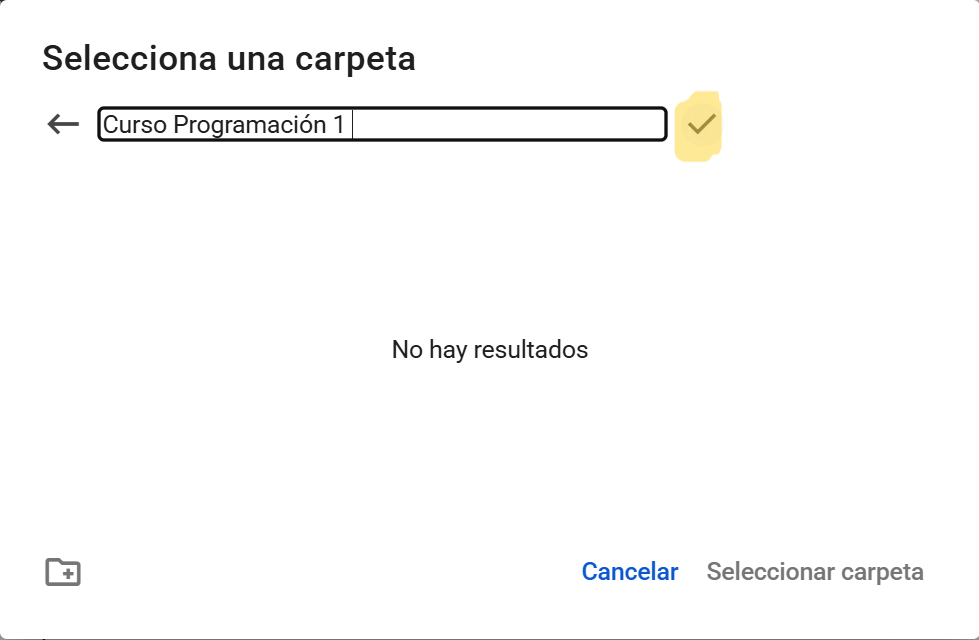
\includegraphics[width=0.95\textwidth]{2) Colab/GColab05.png}
  \end{figure}
\end{frame}

\begin{frame}
  \frametitle{Google Colab - Tutorial Paso a Paso}
  \begin{center}
    \textbf{Paso 6: Selecionar la carpeta creada}
  \end{center}
  \begin{figure}
    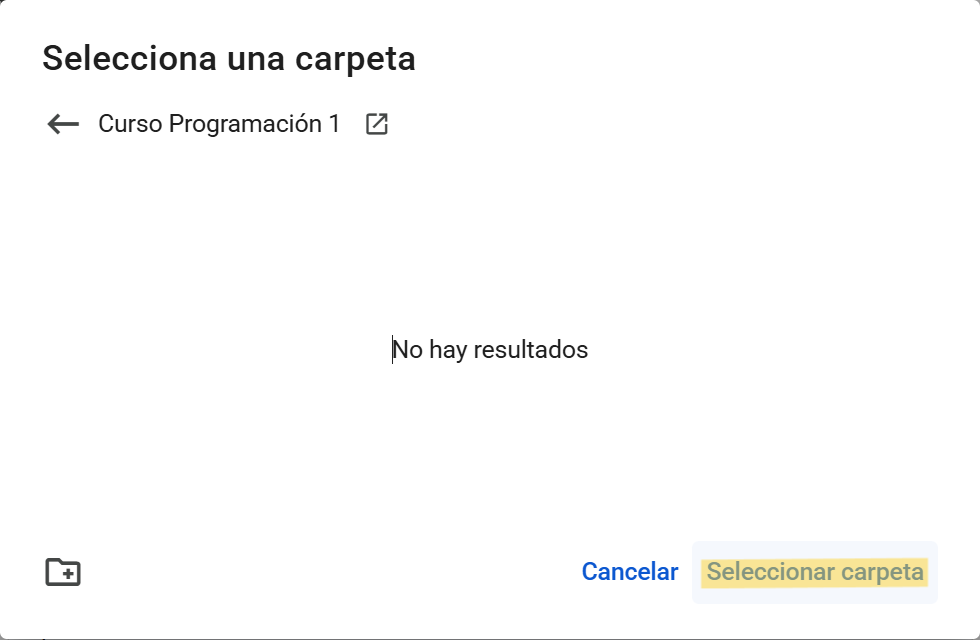
\includegraphics[width=0.95\textwidth]{2) Colab/GColab06.png}
  \end{figure}
\end{frame}

\begin{frame}
  \frametitle{Google Colab - Tutorial Paso a Paso}
  \begin{center}
    \textbf{Paso 7: Darle nombre al notebook}
  \end{center}
  \begin{figure}
    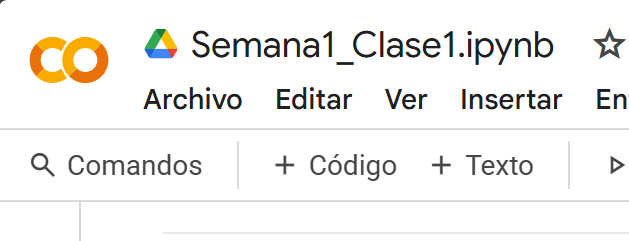
\includegraphics[width=0.95\textwidth]{2) Colab/GColab07.png}
  \end{figure}
\end{frame}

% ------------------------------------------------------------------------
% Slide 7.1: Advertencia sobre IA
% ------------------------------------------------------------------------
\begin{frame}
  \frametitle{Advertencia Importante sobre Inteligencia Artificial}
  
  \begin{columns}
    \begin{column}{0.6\textwidth}
      \begin{alertblock}{¡Cuidado con el abuso de la IA!}
        \begin{itemize}
          \item La IA puede ayudarte a entender conceptos y resolver dudas.
          \item \textbf{PERO} el abuso puede generar problemas en tu aprendizaje.
          \item \textbf{Aprende haciendo}: programa tú mismo, comete errores, debuggea.
          \item La IA debe \textbf{complementar}, no \textbf{reemplazar} tu proceso de aprendizaje.
        \end{itemize}
      \end{alertblock}
    \end{column}
    \begin{column}{0.40\textwidth}
      \begin{figure}
        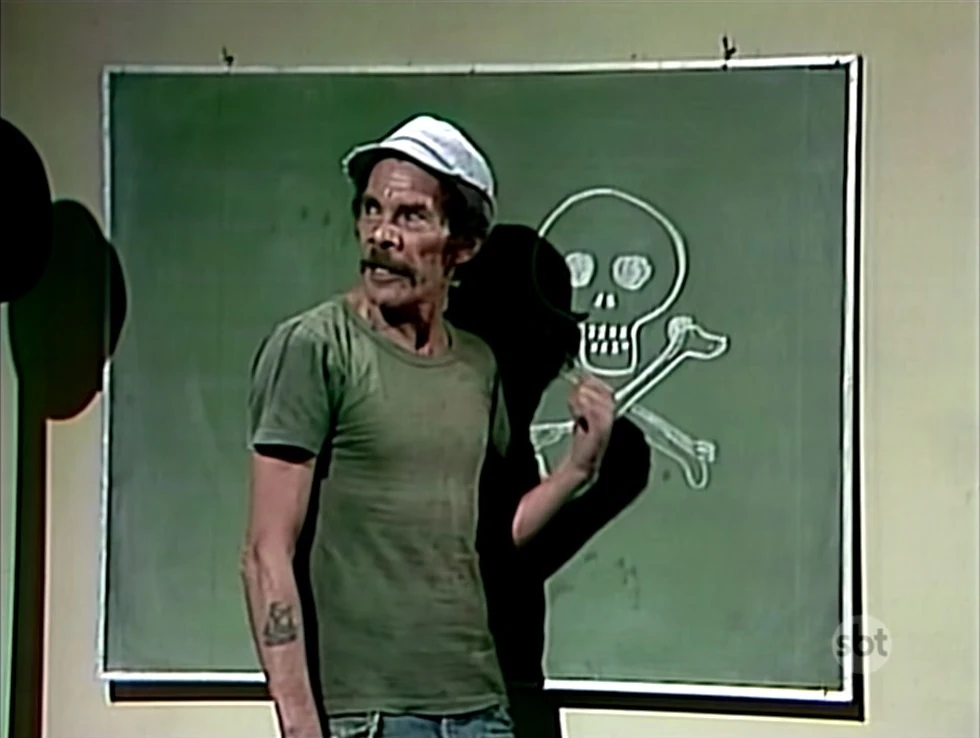
\includegraphics[width=\textwidth]{4) Peligro/Don Ramon.png}
      \end{figure}
    \end{column}
  \end{columns}
\end{frame}


% ------------------------------------------------------------------------
% Slide 8: Ejecución de Código en Colab
% ------------------------------------------------------------------------
\begin{frame}[fragile]{Nuestra Primera Ejecución en Colab}
\begin{minted}{python}
print("¡Hola, mundo de la Física y Astronomía!")
\end{minted}
\begin{itemize}
  \item Presiona \textbf{Shift+Enter} o haz clic en el “play” para ejecutar.
  \item Observa el resultado inmediatamente.
\end{itemize}
\end{frame}

% ----------------------------------------------------------------------------------------
% SECCIÓN 3: Fundamentos de Python
% ----------------------------------------------------------------------------------------
\section{Fundamentos de Python}

% ------------------------------------------------------------------------
% Slide 9: Tipos de Datos y Variables
% ------------------------------------------------------------------------
\begin{frame}{Tipos de Datos y Variables}
  \begin{itemize}
    \item \textbf{int} (enteros), \textbf{float} (reales), \textbf{str} (cadenas), \textbf{bool} (True/False).
    \item En Python, basta con asignar para crear una variable:
          \[
            x = 10 \quad \text{(int)}
          \]
          \[
            saludo = "Hola" \quad \text{(str)}
          \]
    \item \textbf{No se requiere declaración previa} de tipo. Otros lenguajes sí, por ejemplo \texttt{C}, o \texttt{C++}.
  \end{itemize}
\end{frame}

% ------------------------------------------------------------------------
% Slide 10: Nombrado de Variables
% ------------------------------------------------------------------------
\begin{frame}{Reglas de Nombrado de Variables}
  \begin{itemize}
    \item Usar nombres descriptivos (\texttt{masa\_objeto}, \texttt{velocidad\_inicial}, etc.).
    \item No comenzar con dígitos (\texttt{2variable} es inválido, \texttt{variable2} es válido).
    \item \textbf{Distinción de mayúsculas/minúsculas}: \texttt{Radio} vs \texttt{radio}.
    \item Evitar palabras reservadas (\texttt{if}, \texttt{else}, \texttt{class}, etc.).
  \end{itemize}
\end{frame}

% ------------------------------------------------------------------------
% Slide 11: Operaciones Básicas
% ------------------------------------------------------------------------
\begin{frame}[fragile]{Operaciones Básicas con Python}

\begin{minted}{python}
a = 5
b = 2
suma       = a + b     # 7
resta      = a - b     # 3
producto   = a * b     # 10
division   = a / b     # 2.5 (float)
division_entera = a // b # 2 (int)
exponente  = a ** b    # 25 (5^2)
modulo     = a % b     # 1 (resto de la división)
\end{minted}

\begin{itemize}
  \item \texttt{/} produce un resultado float.
  \item \texttt{//} realiza \emph{división entera}.
\end{itemize}

Acá si ejecutamos no veremos los resultados, ya que para mostrar estos resultados en la pantalla, debemos utilizar la función \texttt{print} de python.
\end{frame}

% ------------------------------------------------------------------------
% Slide 12: Entrada y Salida de Datos
% ------------------------------------------------------------------------
\begin{frame}[fragile]{Entrada y Salida de Datos}
\begin{itemize}
  \item \texttt{input()} para capturar información del usuario (devuelve \texttt{str}).
  \item \texttt{print()} para mostrar resultados en pantalla.
\end{itemize}
\begin{minted}{python}
nombre = input("¿Cuál es tu nombre?: ")
print("Hola", nombre, "bienvenido/a al curso!")
\end{minted}

Esta forma de la función \texttt{print} es hoy día mayoritariamente utilizada con \textit{f-string}, lo que sería:

\begin{minted}{python}
  nombre = input("¿Cuál es tu nombre?: ")
  print(f'Hola {nombre} bienvenido/a al curso!')
  \end{minted}

  Para el curso, trataremos de utilizar \textit{f-string}, aunque otras alternativas no estan obsoletas, ni prohibídas.
\end{frame}


\section{Ejercicios Guiados}


% ------------------------------------------------------------------------
% Slide 13: Ejemplo Completo 1
% ------------------------------------------------------------------------
\begin{frame}[fragile]{Ejercicio Guiado 1: Cálculo de Área \\ de un Círculo}
\begin{minted}{python}
import math

r_str = input("Ingresa el radio del círculo: ")
r = float(r_str)
area = math.pi * (r**2)
print(f'El área del círculo es: {area}')
\end{minted}
\begin{itemize}
  \item \texttt{import math} habilita funciones y constantes matemáticas (ej. \texttt{math.pi}).
  \item \textbf{Observación:} Si se introduce un valor no numérico, el programa fallará (manejo de errores).
\end{itemize}
\end{frame}

% ------------------------------------------------------------------------
% Slide 14: Mini-Ejercicio Guiado
% ------------------------------------------------------------------------
\begin{frame}{Ejercicio Guiado 2\hfill \textcolor{red}{$\clubsuit$}}
\begin{block}{Ejercicio}
  \begin{itemize}
    \item Escribe un programa que pida la masa (kg) y la aceleración (m/s\(^2\)).
    \item Calcula la fuerza resultante (\(F = m \times a\)).
    \item Muestra el resultado en pantalla.
  \end{itemize}
\end{block}
\textbf{Tip:} Recuerda convertir la cadena de \texttt{input()} a \texttt{float}.
\end{frame}


% ------------------------------------------------------------------------
% Slide 15: Solución Propuesta
% ------------------------------------------------------------------------
\begin{frame}[fragile]
\frametitle{Solución Propuesta \hfill \textcolor{green}{$\checkmark$}}
\begin{minted}{python}
m_str = input("Ingresa la masa (kg): ")
a_str = input("Ingresa la aceleración (m/s^2): ")

m = float(m_str)
a = float(a_str)
F = m * a

print(f'La fuerza resultante es: {F} N')
\end{minted}
\begin{itemize}
  \item Añadir unidades en la salida (ej.: “N” para Newtons).
  \item Discutir manejo de errores, validación de datos, etc.
\end{itemize}
\end{frame}


% ------------------------------------------------------------------------
% Slide 14.5: Mini-Ejercicio de Depuración
% ------------------------------------------------------------------------
\begin{frame}[fragile]{Mini-Ejercicio de Depuración \hfill \textcolor{red}{$\clubsuit$}}
\begin{block}{¡Encuentra y Corrige los Errores!}
  Copia este código en Colab y ejecútalo. \textbf{¡Tiene errores a propósito!}
\end{block}

\begin{minted}{python}
# Programa para calcular el cuadrado de un número
x = input("Ingrese un número: ")
print("El número ingresado es:", x)
y = x + x
print("El doble del número es:", y)
z = x * x
print("El cuadrado del número es:" z)
\end{minted}


\textbf{Preguntas:} 
\begin{itemize}
  \item ¿Qué errores encuentras?
  \item ¿Cómo los solucionarías?
  \item ¿El resultado es el esperado?
\end{itemize}
\end{frame}

% ------------------------------------------------------------------------
% Slide 14.6: Solución y Explicación de Errores
% ------------------------------------------------------------------------
\begin{frame}[fragile]{Solución y Tipos de Errores \hfill \textcolor{green}{$\checkmark$}}

\textbf{Errores encontrados:}
\begin{enumerate}
  \item \textbf{Error de sintaxis:} Falta comilla de cierre en \texttt{input()}
  \item \textbf{Error de sintaxis:} Falta coma en el último \texttt{print()}
  \item \textbf{Error lógico:} \texttt{input()} devuelve \texttt{str}, no \texttt{int}
\end{enumerate}

\textbf{Código corregido:}
\begin{minted}{python}
# Programa para calcular el cuadrado de un número
x_str = input("Ingrese un número: ")
x = float(x_str)
print("El número ingresado es:", x)
y = x + x  # o también: y = 2 * x
print("El doble del número es:", y)
z = x * x  # o también: z = x ** 2
print("El cuadrado del número es:", z)
\end{minted}

\textbf{Lección:} ¡Los errores son normales! Aprende a leer los mensajes de error.
\end{frame}



% ----------------------------------------------------------------------------------------
% SECCIÓN 4: Actividad Práctica y Ejercicios
% ----------------------------------------------------------------------------------------
\section{Actividad Práctica}

% ------------------------------------------------------------------------
%%%%%%%%%%%%%%%%%%%%%%%%%%%%%%%%%%%%%%%%%%%%%%%%%%%%%%%%%%%%%%%%%%%%%%%%%%%%%%%%%%%%%%%%%%%%%%%%%%%%%%%%%
%%%%%%%%%%%%%%%%%%%%%%%%%%%%%%%%%%%%%%%%%%%%%%%%%%%%%%%%%%%%%%%%%%%%%%%%%%%%%%%%%%%%%%%%%%%%%%%%%%%%%%%%
%\begin{frame}{Problema 1: \hfill \textcolor{red}{$\clubsuit$} \\ Suma de Enteros Consecutivos}
%\begin{block}{Enunciado}
%  \begin{itemize}
%    \item Pedir un número entero \(n\).
%    \item Calcular \(\sum_{k=1}^{n} k\).
%    \item Mostrar el resultado final.
%  \end{itemize}
%\end{block}
%\textbf{Pistas}:
%\begin{itemize}
%  \item Usar un bucle o la fórmula \(\frac{n(n+1)}{2}\).
%  \item ¿Cambios si \(n\) es muy grande?
%\end{itemize}

%Claramente, no hemos revisado bucles, ni cosas similares ya que es nuestra primera clase, pero anímese e investigue online sobre distintas formas de atacar este problema. Más adelante vamos a ir conociendo más sobre python.

%\end{frame}

% ------------------------------------------------------------------------
% Slide 17: Problema 2 (Grupal)
% ------------------------------------------------------------------------
%\begin{frame}{Problema 2: \hfill \textcolor{red}{$\clubsuit$} \\ Cálculo de Energía Cinética}
%\begin{block}{Enunciado}
%  \begin{itemize}
%    \item Dada masa \(m\) y velocidad \(v\), calcular \(E_c = \frac{1}{2}mv^2\).
%    \item Pedir \(m\) y \(v\) repetidamente.
%    \item Detener cuando \(m=0\).
%  \end{itemize}
%\end{block}
%\textbf{Discusión}:
%\begin{itemize}
%  \item ¿Por qué usar \texttt{while}?
%  \item ¿Cómo terminar el bucle de forma limpia?
%\end{itemize}
%\end{frame}
% ------------------------------------------------------------------------
% Slide 18: Trabajo en Equipo
% ------------------------------------------------------------------------
%\begin{frame}{Actividad Práctica}
%\begin{block}{Indicaciones}
%  \begin{itemize}
%    \item Revisen las soluciones de todos.
%    \item Anoten dificultades o errores surgidos.
%    \item Elaboren pequeñas conclusiones o dudas para la clase siguiente.
%  \end{itemize}
%\end{block}
%\end{frame}
%%%%%%%%%%%%%%%%%%%%%%%%%%%%%%%%%%%%%%%%%%%%%%%%%%%%%%%%%%%%%%%%%%%%%%%%%%%%%%%%%%%%%%%%%%%%%%%%%%%%%%%%%%%%%%%%%%
%%%%%%%%%%%%%%%%%%%%%%%%%%%%%%%%%%%%%%%%%%%%%%%%%%%%%%%%%%%%%%%%%%%%%%%%%%%%%%%%%%%%%%%%%%%%%%%%%%%%%%%%%%%%%%%%%%

\begin{frame}{Problema 1: \hfill \textcolor{red}{$\clubsuit$} \\ Conversión de Unidades de Distancia}
\begin{block}{Enunciado}
  \begin{itemize}
    \item Pedir una distancia en metros al usuario.
    \item Convertir a kilómetros, centímetros y milímetros.
    \item Mostrar todos los resultados con sus unidades correspondientes.
  \end{itemize}
\end{block}
\textbf{Pistas}:
\begin{itemize}
  \item Recordar las conversiones: 1 m = 0.001 km, 1 m = 100 cm, 1 m = 1000 mm.
  \item Usar \texttt{f-strings} para mostrar resultados con formato claro.
  \item ¿Qué pasa si el usuario ingresa un número muy grande o muy pequeño?
\end{itemize}

\textbf{Ejemplo esperado:} Si ingresa 5 metros, debería mostrar: 5 m = 0.005 km = 500 cm = 5000 mm.

\end{frame}

% ------------------------------------------------------------------------
% Slide 17: Problema 2 (Grupal)
% ------------------------------------------------------------------------
\begin{frame}{Problema 2: \hfill \textcolor{red}{$\clubsuit$} \\ Calculadora de Velocidad}
\begin{block}{Enunciado}
  \begin{itemize}
    \item Pedir distancia recorrida (en metros) y tiempo empleado (en segundos).
    \item Calcular la velocidad usando \(v = \frac{d}{t}\).
    \item Mostrar el resultado en m/s y como \textbf{bonus} convertir a km/h.
  \end{itemize}
\end{block}
\textbf{Pistas}:
\begin{itemize}
  \item Para convertir de m/s a km/h, multiplicar por 3.6.
  \item Considerar qué pasa si el tiempo es cero (¡división por cero!).
  \item Incluir unidades en la salida para claridad.
\end{itemize}

\textbf{Física relevante:} Esta es una de las ecuaciones cinemáticas más fundamentales.

\end{frame}

% ------------------------------------------------------------------------
% Slide 18: Problema 3 (Grupal) - BONUS
% ------------------------------------------------------------------------
\begin{frame}{Problema 3: \hfill \textcolor{red}{$\clubsuit$} \\ Calculadora de Índice de Masa Corporal}
\begin{block}{Enunciado}
  \begin{itemize}
    \item Pedir peso (en kg) y altura (en metros) al usuario.
    \item Calcular el IMC usando la fórmula: \(IMC = \frac{peso}{altura^2}\).
    \item Mostrar el resultado con interpretación básica.
  \end{itemize}
\end{block}
\textbf{Pistas}:
\begin{itemize}
  \item Usar el operador \texttt{**} para elevar al cuadrado.
  \item IMC < 18.5: bajo peso, 18.5-24.9: normal, 25-29.9: sobrepeso, ≥30: obesidad.
  \item ¿Cómo mostrar el resultado con 2 decimales?
\end{itemize}

\textbf{Aplicación:} Aunque no es estrictamente física, involucra cálculos matemáticos relevantes para ciencias de la salud.

\end{frame}

% ------------------------------------------------------------------------
% Slide 19: Trabajo en Equipo
% ------------------------------------------------------------------------
\begin{frame}{Actividad Práctica}
\begin{block}{Indicaciones}
  \begin{itemize}
    \item Trabajen en equipos de 2-3 personas.
    \item Cada equipo debe intentar resolver al menos los Problemas 1 y 2.
    \item El Problema 3 es opcional (para equipos que terminen rápido).
    \item Prueben sus programas con diferentes valores de entrada.
    \item Anoten cualquier error o comportamiento inesperado que encuentren.
  \end{itemize}
\end{block}

\textbf{Tiempo sugerido:} 20-25 minutos para programar + 10 minutos para discusión grupal.

\begin{alertblock}{Importante}
¡No se preocupen por hacer el código "perfecto"! El objetivo es practicar lo aprendido y familiarizarse con la programación.
\end{alertblock}
\end{frame}


% ------------------------------------------------------------------------
% Slide 19: Retroalimentación y Pausa
% ------------------------------------------------------------------------
\begin{frame}{Retroalimentación}
  \begin{itemize}
    \item ¿Problemas encontrados?
    \item ¿Qué fue lo más intuitivo / confuso?
    \item ¿Dudas para la próxima clase?
  \end{itemize}
  \vspace{0.3cm}
  \textbf{Mantenga estos datos en su cuaderno, le servirá para estudiar.}
\end{frame}

% ----------------------------------------------------------------------------------------
% SECCIÓN 5: Curiosidades y Recursos
% ----------------------------------------------------------------------------------------
\section{Curiosidades y Recursos}

% ------------------------------------------------------------------------
% Slide 20: Breve Historia de Python
% ------------------------------------------------------------------------
\begin{frame}{Pequeña Historia de Python}
  \begin{itemize}
    \item Creado por Guido van Rossum a finales de los 80.
    \item Nombre inspirado en el grupo de comedia \emph{Monty Python}.
    \item Filosofía: legibilidad, sencillez y productividad.
  \end{itemize}
\end{frame}

% ------------------------------------------------------------------------
% Slide 21: Recursos Online
% ------------------------------------------------------------------------
\begin{frame}{Recursos Online}
  \begin{itemize}
    \item \textbf{Para practicar Python:} \href{https://www.hackerrank.com/domains/python?filters\%5Bdifficulty\%5D\%5B\%5D=easy}{HackerRank - Python Practice}
    \item \href{https://www.python.org}{\textbf{python.org}} - Documentación oficial.
    \item \href{https://colab.research.google.com}{\textbf{Google Colab}} - Entorno en la nube.
    \item \textbf{Real Python} (sitio con tutoriales y guías).
    \item \textbf{Stack Overflow} (para consultas y dudas).
  \end{itemize}
\end{frame}

% ------------------------------------------------------------------------
% Slide 22: Comunidades
% ------------------------------------------------------------------------
\begin{frame}{Comunidad y Foros}
  \begin{itemize}
    \item \textbf{Stack Overflow}: millones de preguntas y respuestas.
    \item \textbf{Reddit /r/learnpython}: foros de principiantes.
    \item \textbf{GitHub}: proyectos y ejemplos de ciencia y Python.
  \end{itemize}
  \textbf{Tip:} Buscar soluciones o inspiración es parte del desarrollo como programador.
\end{frame}

% ----------------------------------------------------------------------------------------
% SECCIÓN 6: Conclusiones
% ----------------------------------------------------------------------------------------
\section{Conclusiones}

% ------------------------------------------------------------------------
% Slide 23: Resumen de la Sesión
% ------------------------------------------------------------------------
\begin{frame}{Resumen de la Sesión}
  \begin{itemize}
    \item Configuramos Google Colab y ejecutamos nuestro primer código en Python.
    \item Conocimos los tipos de datos y operaciones aritméticas básicas.
    \item Hicimos ejercicios de entrada/salida y ejemplos físicos sencillos.
    \item Exploramos recursos para continuar aprendiendo.
  \end{itemize}
\end{frame}

% ------------------------------------------------------------------------
% Slide 24: Avances y Próximos Pasos
% ------------------------------------------------------------------------
\begin{frame}{Próximos Pasos}
  \begin{itemize}
    \item \textbf{Unidad II:} Estructuras de control (\texttt{if}, \texttt{for}, \texttt{while}) y funciones en Python.
    \item \textbf{Tarea Sugerida}: 
      \begin{itemize}
        \item Practicar más ejercicios con \texttt{input()} y conversión de tipos.
        \item Explorar \texttt{math}, \texttt{random}, etc.
      \end{itemize}
  \end{itemize}
\end{frame}

% ------------------------------------------------------------------------
% Slide 25: Cierre y Agradecimientos
% ------------------------------------------------------------------------
\begin{frame}
  \huge{\centerline{¡Gracias y hasta la próxima sesión!}}
  \vspace{0.5cm}
  \normalsize
  \begin{itemize}
    \item Revisen la plataforma (Colab) para ejercicios adicionales.
    \item Traigan sus dudas la próxima clase.
  \end{itemize}
\end{frame}

\end{document}

